\documentclass[a4j,dvipdfmx]{jsarticle}

\usepackage[dvipdfmx]{graphicx}
\usepackage{amsmath,amssymb}
\usepackage{siunitx}
\usepackage{ascmac}
\usepackage[subrefformat=parens]{subcaption}
\usepackage{fancyhdr}
\usepackage{otf}
\usepackage[dvipdfmx]{hyperref}
\usepackage{pxjahyper}
\usepackage{okumacro}
\usepackage{tikz}
\usepackage{bm}
\usepackage{ulem}

\usepackage{amsthm}

\usepackage{titlesec}
\usepackage{tocloft} % 目次の設定をカスタマイズするためのパッケージ

\usepackage{makeidx}
\makeindex

% 式番号専用のセクション番号(「\S」を除外)
\newcommand{\plainsectionnumber}{\arabic{section}}

% 式番号にセクション番号を反映
\numberwithin{equation}{section}
\renewcommand{\theequation}{\plainsectionnumber.\arabic{equation}}

\pagestyle{headings}

% \renewcommand{\thesubsection}{\arabic{subsection}}
\renewcommand{\headrulewidth}{1pt}
\renewcommand{\Re}{\operatorname{Re}}
\renewcommand{\Im}{\operatorname{Im}}

% 目次にも「\S」を反映
\renewcommand{\thesection}{\S\arabic{section}}

% tocの番号幅を調整(「\S」で番号が長くなるため)
\setlength{\cftsecnumwidth}{3.5em} % セクション番号の幅を調整



\newcounter{basic_quastion}\setcounter{basic_quastion}{1}
\newcommand{\basicquestion}{\noindent{\large 基本問題\hspace{1mm}\huge\fbox{\textbf{\arabic{basic_quastion}}}\addtocounter{basic_quastion}{1}}\thispagestyle{fancy}\lhead{$\Sigma$基本問題}\rhead{\thepage}\cfoot{}\quad}
\newcommand{\sign}{\mathop{\mathrm{sign}}\nolimits}
\newcommand{\linktoMOKUZI}{\vspace{\stretch{1}}\fbox{\centerline{\hyperref[目次]{目次に戻る}}}}

\newcounter{basic_answer}\setcounter{basic_answer}{1}
\newcommand{\basicanswer}{\noindent{\large 基本問題\hspace{1mm}\huge\fbox{\textbf{\arabic{basic_answer}}}\addtocounter{basic_answer}{1}}\thispagestyle{fancy}\lhead{基本問題解答}\rhead{\thepage}\cfoot{}\quad}

\title{Quuノート -微分積分\ajRoman{2}-}
\date{最終更新 2025/01/10}
\author{責任者 Quu}

\begin{document}
    \maketitle
        \thispagestyle{empty}
    \begin{figure}[h]
        \centering
        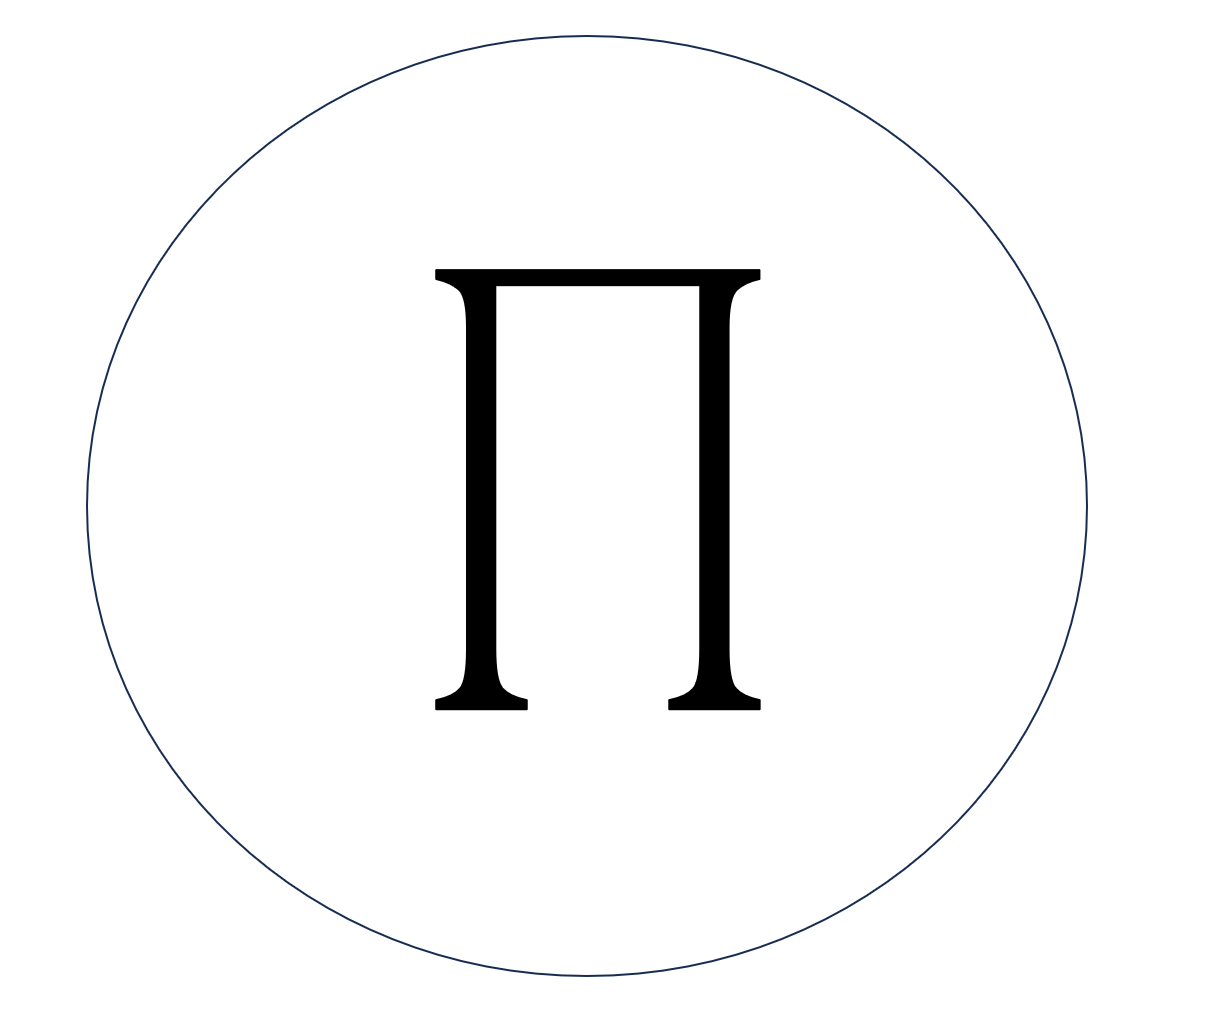
\includegraphics[scale=0.5]{img/QuuNote/QuuNote2/icon.png}
    \end{figure}
    
    \vspace{\stretch{1}}
    \centerline{\textbf{概要}}
    \noindent
    微分積分学入門についてのノート.\\
    主に, 多変数微分積分, ベクトル解析, 複素解析について扱う.
    \clearpage
     
    \clearpage
    \part*{このノートを読む前に}
        このノートは, QuuノートIから引き続き微分積分を学ぶためのノートである. QuuノートIに書いてあることをあらかた身に着けた方なら特別苦も無く読み進められる
        程度の難易度になっている. 前回の思想である厳密さと計算への応用の両立はそのまま受けつがれている. 本ノートでは, 主にIで触れなかった多変数の微分積分
        について述べ, その後ベクトル解析や複素解析について述べる. そして, 物理への応用として, あの相対性理論についてすこしだけ触れ, 現代数学に欠かせない
        Lebesgue積分論についても述べようと思う. こうみると, 微分積分のノートというにはいささか内容が多い. 通常微分積分と言ったら, 最初の多変数の微分積分
        だけを指す. しかしこのノートでは, もっとさまざまな解析学の分野に触れ, それらを大観できる, そんな内容になっているのだ. どちらかといえば, 高木貞二の解析概論
        に近いものになっているだろう. \\

        それぞれの部の内容について, 簡単に紹介しようと思う. 
        
        まず, 第一部では基礎数学について述べる. 具体的には, 集合論の基礎, 線形代数のうち, 行列と行列式について,
        そして, 多変数関数の微分である偏微分と多変数関数の積分である多重積分について述べる. 集合論は, これまで学んできた数学よりも抽象度が高く, 厳密性も求められるから
        初めて学ぶ際は少し戸惑われるだろう. ここはじっくり学んでほしい. 直接の応用としては, 後に述べるLebesgue積分論にかかわってくる. 線形代数は, 正直本ノートでは
        すこしも触れたくなかった話題である. しかし, 多重積分の変数変換において登場するヤコビアンのためには, 行列式の概念が必要であるから, 必要最低限述べた.
        偏微分と多重積分は, 一変数の場合から単純に拡張しただけであるから, すんなり理解できると思う.

        次に, 第二部では, ベクトル解析について述べる. ベクトル解析で扱われる豊富な内容のうち, 重要なものをかいつまんで扱う. ベクトル値関数の微分積分はもちろん, 
        平面そして空間上の曲線の解析も行う. また, 曲面についても解析を行う. これらの内容は,  微分幾何に通じるもので, 一般相対論でも重要である. その後, 場の概念について
        扱う. これは物理, 特に電磁気学との関連の深いから, 電磁気学の例を用いて説明する. その後, ベクトル場上の積分定理についても扱う. いわゆるGaussの定理やStokesの定理である.
        総じて, この部における数学は, ほかの部の数学に比べて厳密性を無視した展開となっているから注意してほしい. しかし, 厳密性を多少犠牲にしてでも, 明快に解説できたと思う.

        次に, 第三部では, 複素解析について扱う. 複素数について簡単な性質を述べたのち, 複素関数を定義する. 複素関数に対しても, 実数の場合と同様微分積分が定義できて, とくに
        微分可能性に対して, 実数よりも少し厳しい条件を付けることで, 実り豊かな結果を得ることができる. 複素解析は, それ自身興味深い対象であるが, 直接的な応用としては, 留数定理
        の存在があるだろう. 実数における定積分を, 複素積分に直すことで, 留数と呼ばれる値の和として表すことができるのだ. 留数は不定積分を経由しない方法で求めることができるので, 不定積分
        ができなくても, 定積分の計算をすることができるというわけである. また, Riemann面を用いて多価関数を扱う方法についても少しだけ述べようと思う.

        第四部では, 相対性理論についてすこしだけ扱う. 一般相対性理論で扱う数学は高級なRiemann幾何学であるが, 特殊相対性理論で扱う数学は簡単な微分積分で十分なのであるから, 学ぶための準備は十分できているといえるだろう.
        まず, 特殊相対性理論について, 入門的に学ぶ. ここで, 相対性理論で用いる諸概念の説明も行う. この時生じるであろうパラドクスについては, つぎのパラドクスの解決で理解していく.
        その後, 相対性理論を適用した力学を展開するための数学について簡単に学ぶ. ここで, 変分法や, ベクトル, テンソルの座標変換についても簡単に述べる. こうして必要な数学を身に着けたら, 
        いよいよ相対性理論を用いた力学について考えていく. このとき, 世界一有名な数式とも言ってよい$E=mc^2$も導出するから楽しみにしていてほしい. また, 前に解決したパラドクスについても, 別の視点から解決することができることを述べる.
        最後に, 一般相対性理論について, その内容を覗いてみる.

        最後に, 第五部では, Lebesgue積分論について簡単に学ぶ. これまで学んできた積分をRiemann積分というが, 実はRiemann積分では様々な制約があった. まず一つ, Riemann積分
        では, 関数が連続でない場合, 積分可能であるとは限らない. 実際関数が有界であって原始関数を持っても, その関数が積分可能であるとは限らない例が存在している. 次に, 積分記号と極限の
        入れ替えのためには, 関数列が一様収束しなければならない. これはIにて学んだことである. 一様収束は, 正直言ってかなり厳しい条件であろう. そんな条件が満たされていないと, 項別に
        積分できないのは, Riemann積分の大きな欠点であるし, 制約である. それに対して, Lebesgue積分では, これらの制約が大幅に緩和される. 例えば, 関数列$\{f_n\}$が区間$[a,b]$の各点で
        $\lim f_n=f$であるとき, すべての$n$に対して$|f_n(x)|<M$となる定数$M$が存在すれば, $\lim\int f_n(x)dx=\int f(x)dx$とできるのだ(まさに項別積分!!). 
        流れとしては, まず考察したい全体の集合に対して,扱う部分集合の対象として都合の良いものを集めた$\sigma$-集合体というものを定義する. この$\sigma$集合体と全体集合を用いて
        可測空間なるものが作られる. その集合体内に含まれる部分集合はすべて可測集合と呼ばれ, 可測集合であれば, それに対して測度が定義できる. 測度は, 簡単に言えば, ものの長さや
        立体の体積などを抽象化したもので, 可測空間にこの測度を加えて測度空間を作ることができる. 一方, 全体集合に対して実数を対応させる関数のうち, ある条件をみたすものを可測関数と定義する.
        常に正の値を取る可測関数には, 単関数とよばれる関数の単調増加列が存在して, その収束関数として表すことができるという性質がある. このようにして数学の準備を整えることで, ようやく
        積分が定義できる. 積分を定義し, 基本的な性質について述べた後は, 本命の収束定理について述べていく. これだけの内容を全てしっかり学ぼうとしたら, それだけで一冊できてしまうから, 
        必要最低限のみ解説してこうと思う.\\

        今回のQuuノートIIはIと比べて書式が変わっているところがあるから, 始めに紹介しておく. まず, 定理の名前等に出てくる海外の人名は, すべて英語にしてある.
        これは, 専門的な本ではたいてい人名が英語で書かれていること考慮している. また, 句読点を「、」「。」から「,」「.」に変更した. これも, 理工系の本では後者の方を用いられているからそれに合わせた形となる.
        各節(section)番号の前には\S 記号を付けた. 

        各節ごとに, 基本問題を用意している. これらは是非とも自分で解いてもらいたい. ノートの最後のほうに解答もつけているから, 適宜参照してほしい. Iでも述べたように, これを読んで一度ですべてを理解できなくてもよいし, 
        またその必要もない. ただ, 寝転がりながら読んでも理解できるほど簡単な内容でもない. 紙と鉛筆を用意して, しっかりと繰り返し読んで考えることで, 必ず微分積分が理解できるようになるだろう. 

        これを読んで, 少しでも解析学を大観できたと感じられたら幸いである.\qed\\

        以下に, 各部の関係を示す図をのせる. 参考にしてほしい. 破線の矢印は, 読んでおくと便利というだけで, 読まなくてもあまり困ることはないだろう.
        \begin{figure*}[h]
            \centering
            \begin{tikzpicture}
                \draw (0,0) node[draw,rectangle]{第I部 基礎数学};
                \draw (-4,-1) node[draw,rectangle]{第II部 ベクトル解析};
                \draw (0,-1) node[draw,rectangle]{第III部 複素解析};
                \draw (5,-1) node[draw,rectangle]{第V部 Lebesgue積分入門};
                \draw (-4,-2) node[draw,rectangle]{第IV部 相対性理論};

                \draw[->] (0,-0.3) -- (-4,-0.7);
                \draw[->] (0,-0.3) -- (0,-0.7);
                \draw[->] (0,-0.3) -- (5,-0.7);
                \draw[->] (-4,-1.3) -- (-4,-1.7);
                \draw[->,dashed] (-2.3,-1) -- (-1.5,-1);
            \end{tikzpicture}
        \end{figure*}

        このノートを書く際に使ったアプリケーション等をあげておく.
        \begin{enumerate}
            \item \TeX (正確には\LaTeX)
            \item Tikz (\TeX のパッケージ. 作図するときに便利である.)
            \item VSCode(テキストエディタ.)
            \item PowerPoint(表紙のアイコンを作成するために用いた.)
            \item \href{https://www.wolframalpha.com/}{WolflamAlpha}(検算で大活躍した.)
        \end{enumerate}

        なお, 誤植等があれば遠慮なく連絡してほしい. 質問も大歓迎である.
    \clearpage
    \label{目次}
    \tableofcontents
    \clearpage

    \part{基礎数学}
    \vspace{\stretch{1}}
    \begin{screen}
        ここでは, 数学をするうえで必要となる最低限の基礎知識を学ぶ. 主に, 集合論基礎, 線形代数のうちベクトル, 行列, 行列式の基礎が含まれる.
        また, 多変数関数について微分・積分を定義する. いわゆる偏微分, 重積分というもので, これらの概念を習得することは, 数学, 物理, 工学を学ぶ上で重要である.
    \end{screen}
    \clearpage
    \section{集合論基礎}
        集合とその演算, 写像, 濃度について軽く触れ, 実数論についても少し触れる.
        \subsection{集合とは}
            \textbf{集合}\index{しゅうごう@集合}とは端的に言えば, \underline{ものの集まり}\footnote{素朴な疑問だが, もののあつまりというものはどういうものであろうか. なんだか曖昧な定義である. 例えば, $A\in A$を満たす$A$は集合といえるだろうか.
             この答えはNoであって, それは集合を厳密に定める公理系によって示される. これらの研究は公理的集合論という20世紀に発展した数学の分野の一つである.}である. 実数の集まりでも整数の集まりでもよいし, 関数の集まりでもよい.
            もっと具体的に, 犬, 猫, 人間, など, ともかく何かを集めた集まりである. ある集合に対して, あるものがその集合に含まれていた場合, 
            そのものを集合の\textbf{要素}\index{ようそ@要素}や\textbf{元}\index{げん@元}という. 集合を構成するものといってもよいだろう. $a$が集合$A$の要素であることを次のように表記し, $a$
            は$A$に属するという.
            \begin{equation}
                a \in A \text{または} A \ni a \label{eq:集合論基礎:元の表記}
            \end{equation}
            また, $a$が$A$の要素でないことは$a\not\in A$または$A \not\ni a$と表記する. 例えば, $A$が6の約数全てであるとき, 
            $1\in A,2\in A$であるが, $5\not\in A$である. なお, 集合が集合たるためには, その集める範囲が明確に定義できていなければならない.
            例えば, 学校内の美人な学生全体の集まりは, 美人の定義が定まっていないから集合ではないのである. 大きい服すべての集まり, おいしい食べ物全体の集まり
            なども同様の理由で集合ではない. \\
        
            集合はものの集まりであるから, その要素の個数について気になるところである. 要素の個数が0か自然数で表せる集合を\textbf{有限集合}\index{ゆうげんしゅうごう@有限集合}といい, 
            それ以外の集合を\textbf{無限集合}\index{むげんしゅうごう@無限集合}という. また, 要素の個数が0, すなわち要素を何も持たない集合を\textbf{空集合}\index{くうしゅうごう@空集合}といい, $\varnothing$とかく.
            有限集合としては例えば先ほど例に挙げた6の約数全ての集合がある. 無限集合としては, 自然数全体の集合, 実数全体の集合などがある.

            様々な集合を考えることができるが, 特別な記号で表せる集合があるから紹介しておこう. これらは一般的に, たいてい断りなく用いられる.
            \begin{align*}
                \mathbb{N}&=\text{自然数全体の集合}\\
                \mathbb{Z}&=\text{整数全体の集合}\\
                \mathbb{Q}&=\text{有理数全体の集合}\\
                \mathbb{R}&=\text{実数全体の集合}\\
                \mathbb{C}&=\text{複素数全体の集合}\\
            \end{align*}
            集合を表す方法として, その要素をすべて書き並べる表し方がある. これを\textbf{列記法}\index{れっきほう@列記法}または\textbf{外延的記法}\index{がいえんてききほう@外延的記法}という.
            これを用いて, 先ほど例示した6の約数全ての集合を表す.
            \begin{equation}
                A=\{-6,-3,-2,-1,1,2,3,6\} \label{eq:集合論基礎:列記法の例}
            \end{equation}
            もちろん, 元を書き並べる順序をかえても同じ集合である. また, 重複して書かれた要素は一つのものとして考え, 同じ要素を重複して書くようなことはしない.
            しかし, 要素の数が多くなれば, 要素を全て並べて書くことは困難になることは容易に想像できる. 例えば100万以下の自然数すべての集合を列記法でかく作業は途方もないだろう.
            そこで, 集合の要素となる条件(範囲, 性質)を書いて, それを満たす要素全体として集合を表す方法も存在する. これを\textbf{説明法}\index{せつめいほう@説明法}や\textbf{内包的記法}\index{ないほうてききほう@内包的記法}という.
            これを用いて先ほどの\eqref{eq:集合論基礎:列記法の例}を書くと
            \begin{equation}
                A=\{x\mid\text{$x$は6の約数全体}\} \label{eq:集合論基礎:説明法の例}
            \end{equation}
            となる. このように, 説明法では集合を要素$x$の条件$P(x)$を用いて$\{x\mid P(x)\}$とかく. また, \eqref{eq:集合論基礎:説明法の例}は$\{x\in\mathbb{Z}\mid\text{$x$は6の約数全体}\}$
            とも書かれる. 最初の$x$の前に大前提の$x\in\mathbb{Z}$を書くのである. このほかにも, 特別な集合の場合は固有の表し方もある. 例えば, 閉区間, 開区間の表し方がそうである.\\

            義務教育中に習ったように, 自然数$\mathbb{N}$のすべての要素は整数$\mathbb{Z}$に含まれている. これは, $\mathbb{N}$が$\mathbb{Z}$に`包まれている'ような状態であると理解できる.
            一般に, 二つの集合$A,B$について, $A$の\underline{全ての}要素が$B$の要素であるとき, $A$は$B$の\textbf{部分集合}\index{ぶぶんしゅうごう@部分集合}であるといい,
            \begin{equation}
                A \subset B \text{または} B \supset A \label{eq:集合論基礎:部分集合の表記}
            \end{equation} 
            とかく. この場合, $A$は$B$に\textbf{包まれている}, または$B$は$A$を\textbf{包む}という. 反対に, $A\subset B$ではないことを$A\not\subset B$とかく.
            明らかに, $A\subset A$である. また, $A\subset B,B\subset C$ならば$A\subset C$であることも, 明らかであろう. 
            $A\subset B$かつ$A \supset B$であるとき, $A=B$とかき, 二つの集合$A,B$は\textbf{等しい}という.

            $A\subset B$かつ$A\neq B$であるとき, $A$は$B$の\textbf{真部分集合}\index{しんぶぶんしゅうごう@真部分集合}であるといい, これを強調したい時$A\subsetneq B$とかく. 例えば, $\mathbb{N}$は$\mathbb{Z}$
            の真部分集合である.\\

            集合$A$に対して, $A$の部分集合全体の集合を$A$の\textbf{巾集合}\index{べきしゅうごう@巾集合}といい, $\mathfrak{P}(A), \mathcal{P}(A), 2^{A}$のようにかく.本ノートでは, 最後の記法$2^{A}$を採用することにする.
            巾集合は, その要素全てが集合である. 一般に, どの要素も集合であるような集合を\textbf{集合族}\index{しゅうごうぞく@集合族}という.\footnote{集合族は, 一般にドイツ文字や花文字で表される慣習がある.}

            例えば, $A=\{1,2,3\}$のとき$2^{A}=\{\varnothing,\{1\},\{2\},\{3\},\{1,2\},\{1,3\},\{2,3\},\{1,2,3\}\}$である. 空集合が入っていることに疑問が浮かぶ人もいるだろうから説明しておこう.
            空集合とは, 要素を一つも持たない集合であるから, 論理として「$a$が$A$に含まれていない」ならば「$a$は$\varnothing$に含まれていない」が任意の集合$A$に対して成り立つ.
            実際, 前半の「」の真偽にかかわらず成り立つから, これは正しいと納得されるだろう.\footnote{これは次小節を見ることでより納得がいくはずである.} 
            このときこの命題の対偶\footnote{次小節参照.}を取れば, 「$a$が$\varnothing$に含まれている」ならば「$a$は$A$に含まれている」が成り立つ.
            すなわち, 空集合は任意の集合の部分集合であることがわかる. 
        \clearpage
        \subsection{記号論理}
            ここでは集合論を展開するために便利な記号論理について必要最小限に留めて述べる.

            一般に, 数学の定理は
            \begin{equation}
                p\Rightarrow q \quad (\text{$p$ならば$q$}) \label{eq:集合論基礎:数学の定理の構造}
            \end{equation}
            の形をしていることが多い. $p$をこの定理の\textbf{仮定}, $q$を\textbf{結論}という. $p,q$のように, 真偽の定まる文章を\textbf{命題}\index{めいだい@命題}という.
            命題によっては, それ自身がある複数の命題によって構成されている場合がある. 例えば, $a=1$かつ$b=2$は$a=1$という命題と$b=2$という命題が「かつ」
            によって結合されている. このように, 数学に現れる命題を結合するものは, 次の三種類がある.
            \begin{equation*}
                p\land q,\quad p \lor q,\quad p \Rightarrow q 
            \end{equation*}
            $\land$は「かつ」, $\lor$は「または」, $\Rightarrow$\footnote{$p\Rightarrow q$はこの命題が真であるとすでに分かっているときによく用いられる. まだこの命題が真であるかがわかっていない場合などは$p\rightarrow q$と書いて区別する.}は「ならば」を表す.\footnote{$\land$を論理積, $\lor$を論理和という.} 特に, $p\Rightarrow q \land p \Leftarrow q$であるとき, 
            $p$と$q$は\textbf{同値}\index{どうち@同値}であるといい, $p \Leftrightarrow q$とかく.

            次に, 命題の否定を考える. 命題$p$に対して, その\textbf{否定}\index{ひてい@否定}は「$p$でない」となり, これを$\lnot p$とかく. 以上で紹介した記号$\land,\lor,\lnot,\Rightarrow,\Leftrightarrow$
            を論理演算子という. 命題の合成命題を否定する際には, 書き方に注意を払う必要がある. 例えば, $p\land q$という命題を否定するときに$\lnot p\land q$と書いてはいけない.
            この場合, 「$p$ではない」かつ$q$であるという命題になっているからである. 正しくは, $\lnot(p\land q)$とかく.

            ある命題が真である場合や偽である場合に, それを数値で表すことができたら便利である. そこで, 命題が真である場合, その命題の\textbf{真理値}\index{しんりち@真理値}は1であるといい, 
            偽のとき, その命題の真理値は0であるということにする. 例えば, $p,q$の真理値がそれぞれ$1,0$であるとき, $p\land q$の真理値は$1$である.
            この時重要なのは, $p\land q$の真偽を判断するときに, \underline{$p\land q$の命題の意味を解釈することなく, $p,q$の真偽だけから判断できた}ということである.
            よって, 命題$p_1,p_2,\dots,p_n$の合成命題$p$が与えられたときは, $P$の真偽に重要なのは論理式の構造と$p_1,p_2,\dots,p_n$の真偽だけということになる.


            そこで, 各命題$p_1,p_2,\dots,p_n$の真理値のすべての組み合わせについて$P$を計算した表を考え, これを$P$の\textbf{真理値表}\index{しんりちひょう@真理値表}という. 以下に$p\land q$の真理値表を示す.
            \begin{table}[h]
                \centering
                \begin{tabular}{cc|c}
                    $p$ & $q$ & $p\land q$ \\\hline
                    0 & 0 & 0 \\\hline
                    0 & 1 & 0 \\\hline
                    1 & 0 & 0 \\\hline
                    1 & 1 & 1 \\\hline
                \end{tabular}
                \caption{$p\land q$の真理値表}
            \end{table}

            二つの合成命題$P,Q$が与えられたとき, 真理値表において$P,Q$の真理値表が一致するとき, $P$と$Q$は論理的に\textbf{同値である}\index{どうち@同値}といい, $P\equiv Q$とかく. 試しに, $\lnot (p\land q)$と$(\lnot p)\lor (\lnot q)$
            が論理的に同値であることを示してみる. (次ページ)
            \clearpage
            以下の表を見ればわかるように, $\lnot (p\land q)$と$(\lnot p)\lor (\lnot q)$の真理値はすべて一致している. これより直ちにこれら二つの論理が同値であることがわかる.

            \begin{table}[h]
                \centering
                \begin{tabular}{cc||cc|ccc}
                    $p$ & $q$ & $p\land q$ & $\lnot(p\land q)$ & $\lnot p$ & $\lnot q$ & $(\lnot p)\lor(\lnot q)$ \\\hline
                    0 & 0 & 0 & 1 & 1 & 1 & 1\\
                    0 & 1 & 0 & 1 & 1 & 0 & 1\\
                    1 & 0 & 0 & 1 & 0 & 1 & 1\\
                    1 & 1 & 1 & 0 & 0 & 0 & 0\\
                \end{tabular}
                \caption{真理値表による命題の比較}
            \end{table}

            上記の方法とまったく同様にして, $\lnot (p\lor q)$と$(\lnot p)\land (\lnot q)$が示されるから, 以下の\textbf{De Morganの法則}\index{De Morganのほうそく@De Morganの法則}が成り立つことがわかる.
            \begin{align}
                \lnot (p\land q) \equiv (\lnot p) \lor (\lnot q) \label{eq:集合論基礎:論理ドモルガン1}\\
                \lnot (p\lor q) \equiv (\lnot p) \land (\lnot q) \label{eq:集合論基礎:論理ドモルガン2}
            \end{align}
            De Morganの法則は最も基本的な論理演算の法則であるから, しっかり理解しておこう. この二つの式から双対性の概念が見えるがここでは触れない.

            De Morganの法則を用いれば, $\land,\lor$の含まれる合成命題については否定できるが, $\Rightarrow$が含まれた命題を否定する際はどうすればよいだろうか.
            一度ここでもっとも簡単な形である$p \Rightarrow q$について考察してみよう. すぐわかるのは pが真の場合, $q$が真ならば真, 偽ならば偽
            であるとなることである. 問題は$p$が偽の場合である. このとき$q$が成り立っていようがいまいが(仮定がそもそも偽であるから)真偽には関係のないような気がする.
            そこで\underline{$p$が偽のときには$p\Rightarrow q$は偽である}と定めることにしよう. このように定めるのは, 例えば
            「任意の自然数$n$に対して$n>2\Rightarrow n > \sqrt{5}$」という命題を考える際に便利だからである. 普通に考えてみればこの命題はもちろん真なのであるが, 
            これまでの考え方に則ると, $n=2$のとき「$2>2\Rightarrow 2>\sqrt{5}$」が真でなければならない. なぜなら$n$は\.{任}\.{意}\.{の}自然数だからである. このような場合, 
            下線部のように定めることで, 任意の自然数に対して命題が真であるようにできるのだ. よって, $p\Rightarrow q$の真偽は$\lnot p\lor q$の真偽と一致することがわかる.
            よって, $\lnot (p\Rightarrow q)\equiv \lnot (\lnot p\lor q)\equiv \lnot(\lnot p) \land (\lnot q)\equiv p\land (\lnot q)$となる. ここで, $\lnot (\lnot p)\equiv p$であることを
            用いた. これは真理値表を用いて簡単に示せる.
            以上をまとめると
            \begin{equation}
                \lnot (p \Rightarrow q) \equiv p \land (\lnot q) \label{eq:集合論基礎:ならばの否定}
            \end{equation}
            が得られる. \\

            二つの命題$p,q$に対して, $p\Rightarrow q$が正しくても$q\Rightarrow p$が正しいとは限らない. 例えば, 微分可能であるならば連続であるが, 連続で会っても微分可能ではない
            のが好例である.  $q\Rightarrow p$を$p\Rightarrow q$の\textbf{逆}といい, $\lnot q\Rightarrow \lnot p$を\textbf{対偶}という.
            今述べたように, 命題$p\Rightarrow q$が真であっても逆は真であるとは限らないが, 対偶についてはどうだろうか. 対偶の論理式を式変形してみると
            $\lnot q\Rightarrow \lnot p\equiv \lnot (\lnot q) \lor (\lnot p) \equiv q \lor (\lnot p)\equiv p \Rightarrow q$となる. \footnote{何も言わず$p\lor q \equiv q \lor p$を用いてしまったが, 本来は真理値表で確かめる必要がある. ただ, 直感的に明らかであろう.}
            すなわち, $p \Rightarrow q$とその対偶の真偽は一致する. これは, $p \Rightarrow q$の命題を証明する際には, その対偶を証明してもよいということを示している.
            \clearpage
            最後に, 限定記号について述べておこう. これはこれから多く出てくるからしっかり理解しよう. 変数を含む文章で, 変数に値を代入する値
            と命題になるものを命題関数や述語という. 命題も命題関数も含めて単に命題とよぶ. 例えば, $p(x)\equiv\text{$x$は2と等しい}$という命題関数を考えてみる. ここに$x=2$を代入した命題$p(2)\equiv\text{$2$は2と等しい}$は真である.
            一方$x=1$を代入した命題$p(1)$は偽である.\\

            ここで気になってくるのが, ある命題関数を考えたときに, この命題は全ての$x$について成立しているのか, それともある$x$について成立しているかであろう. 
            このときの「全ての(任意の)」や「ある(或る)」という言葉を\textbf{限定語}\index{げんていご@限定語}という. 例えば, 「三角形の内角の和は$180^\circ$」という命題は「全ての三角形」に対して
            成立している. この「全ての」や「ある」を表す記号として, $\forall,\exists$がある. それぞれ`For all'または`For any', `Exist'に由来する記号で, 
            前者を全称記号\index{ぜんしょうきごう@全称記号}, 後者を存在記号\index{そんざいきごう@存在記号}という. これらをまとめて限定記号\index{げんていきごう@限定記号}という. これを用いて, 全ての実数に対しその平方が0または正であるという命題は$^\forall x\in \mathbb{R} [x^2\geq 0]$と書ける.
            また, 実数全体で定義された関数$f(x)$に対して, $f(x)=x$となる実数$x$が存在するという命題は$^\exists x\in \mathbb{R}[f(x)=x]$と書ける.

            限定記号を用いれば, $\varepsilon-N$論法による極限の定義を簡単な論理式で書くことができる. 試しに, 数列$\{a_n\}$が$a_n\rightarrow \alpha$となることを限定記号を用いて書いてみると
            \begin{equation*}
                {}^\forall \varepsilon>0, {}^\exists N>0, {}^\forall n\in \mathbb{N} \left[n>N \Rightarrow |a_n-\alpha|<\varepsilon\right]
            \end{equation*}
            となる. この書き方のほうがどの変数が何に依存しているかがすっきりしていて見やすいと思う.\\

            最後に, 全称記号および存在記号付きの命題を否定すると, それらが互いに入れ替わることを証明なしに述べて終わる.
            \begin{align}
                \lnot\left({}^\forall x\in X \left[p(x)\right]\right) \equiv {}^\exists x\in X \left[\lnot p(x)\right] \label{eq:集合論基礎:forallの否定}\\
                \lnot\left({}^\exists x\in X \left[p(x)\right]\right) \equiv {}^\forall x\in X \left[\lnot p(x)\right] \label{eq:集合論基礎:existの否定}
            \end{align}
            しかし, これは直感的には理解しやすい. 例えば\eqref{eq:集合論基礎:forallの否定}であれば, 任意の$x$について成り立っていることを否定するのだから, (少なくとも一つは)
            成り立たないような$x$が存在しなければならない. そして, この式に両辺否定を取れば\eqref{eq:集合論基礎:existの否定}がすぐさま導かれる.
        \clearpage
        \subsection{集合の演算}
            集合に話を戻す. 二つの集合$A,B$について, その和と積に対応するものを考えよう. それらは以下のように定められる.
            \begin{align}
                A\cup B = \{x\mid x\in A \lor x \in B\} \label{eq:集合論基礎:和集合の定義}\\
                A\cap B = \{x\mid x\in A \land x \in B\} \label{eq:集合論基礎:共通部分の定義}
            \end{align}
            集合$A\cup B$を$A$と$B$の\textbf{和集合}\index{わしゅうごう@和集合}といい, $A\cap B$を$A$と$B$の\textbf{共通部分}\index{きょうつうぶぶん@共通部分}という. 定義から明らかに次式が成り立つ.
            \begin{align}
                A\subset A \cup B,\quad B\subset A \cup B \label{eq:集合論基礎:和集合の包含関係}\\
                A \cap B \subset A,\quad A \cap B\subset B \label{eq:集合論基礎:共通部分の包含関係}
            \end{align}
            しかし, せっかく記号論理を学んだのだから, 上式を証明してみるのもよいだろう. 試しに, \eqref{eq:集合論基礎:和集合の包含関係}を示してみることにしよう.
            対称性から, 示すべき命題は, $x\in A \rightarrow x\in A \cup B$で十分である. $x \in A \rightarrow x \in A \lor x\in B$であり, 右辺は和集合の定義そのもの
            だから, 示された. やはり明らかであったが, 簡単な命題でも記号論理の威力が垣間見えるだろう.

            二つの集合が共通の要素を一つも持たない場合, 共通部分に含まれる要素は存在しない. この場合, 要素数は0であるから空集合である. 集合$A,B$に対し, $A\cap B =\varnothing$であるとき,
            $A$と$B$は\textbf{交わらない(互いに素である)}\index{たがいにそ@互いに素}という. 逆に, $A\cap B\neq \varnothing$のとき, 二つの集合は交わるという.\\

            集合演算の基本的な性質について述べよう. 以下に式を列挙する.
            \begin{align}
                &A\cup B = B \cup A, \quad A \cap B = B \cap A \label{eq:集合論基礎:和集合と共通部分の交換法則}\\
                &(A\cup B)\cup C = A\cup (B \cup C) \label{eq:集合論基礎:和集合の結合法則}\\
                &(A\cap B)\cap C = A\cap (B \cap C) \label{eq:集合論基礎:共通部分の結合法則}\\
                &A\cup (B \cap C) = (A\cup B) \cap (A\cup C)\label{eq:集合論基礎:和を積に直す分配法則}\\
                &A\cap (B \cup C) = (A\cap B) \cup (A\cap C)\label{eq:集合論基礎:積を和に直す分配法則}
            \end{align}
            \eqref{eq:集合論基礎:和集合と共通部分の交換法則}は\textbf{交換法則}, \eqref{eq:集合論基礎:和集合の結合法則}, \eqref{eq:集合論基礎:共通部分の結合法則}は\textbf{結合法則}, \eqref{eq:集合論基礎:和を積に直す分配法則}, \eqref{eq:集合論基礎:積を和に直す分配法則}
            は\textbf{分配法則}である. これらはすべて定義から記号論理を駆使して簡単に証明できる. ここでは, \eqref{eq:集合論基礎:和を積に直す分配法則}のみ証明することにする.
            \begin{proof}
                示すのは, $x\in A\cup (B \cap C) \leftrightarrow x\in (A\cup B) \cap (A\cup C)$である.
                $x\in A\cup (B \cap C) \leftrightarrow x\in A \lor x\in B\cap C \leftrightarrow x\in A \lor (x\in B \land x\in C)$であるから, 命題に関する分配法則が成立すればよい.
                真理値表を書けばわかるように, $p\lor (q\land r)\equiv (p\lor q) \land (p\lor r)$だから, $x\in A\cup (B \cap C) \leftrightarrow (x\in A\lor x\in B)\land (x\in A\lor x\in C)\leftrightarrow x\in A\cup B\land x\in A\cup C\leftrightarrow x\in (A\cup B)\cap (A\cup C)$
                となる. 以上より, \eqref{eq:集合論基礎:和を積に直す分配法則}が示された.
            \end{proof}

            二つの集合$A,B$に対して, 差に対応するものを考える. これは以下のように定義する.
            \begin{equation}
                A-B = \{x\mid x\in A \land x\not\in B\} \label{eq:集合論基礎:差集合の定義}
            \end{equation}
            集合$A-B$を$A$と$B$の\textbf{差集合}\index{さしゅうごう@差集合}という. 一般に, $A-B\neq B-A$である. 等号が成り立つのは$A=B$の場合のみである. これは実数の場合と同様であるから理解しやすい.\\

            数学では, ある集合を基礎として, その要素について考察する場合が多い. 例えば, QuuノートIでは実数の集合$\mathbb{R}$において, その微分積分等を考察していた.
            このような, 特定の集合$\Omega$の要素と部分集合について議論する場合, $\varOmega$を\textbf{全体集合}\index{ぜんたいしゅうごう@全体集合}という. 全体集合にはよく$\varOmega,U$といった記号が用いられる.
            全体集合$\varOmega$が与えられたとき, 考察の対象となる集合$A\subset \varOmega$に対して, $\varOmega - A$を考えることができる. 
            この差集合$\varOmega - A$を$\varOmega$における$A$の\textbf{補集合}\index{ほしゅうごう@補集合}といい, $A^c$とかく.\footnote{cはcomplementの頭文字.}
            任意の$x\in \varOmega$に対して, $x\in A^c \Leftrightarrow x\not\in A$が成立する.

            以降, 特別断りがない場合$\varOmega$を全体集合とする. 任意の$A\subset \varOmega$に対して, 以下が成り立つ.
            \begin{align}
                &(A^c)^c = A\\
                &A\cup A^c = \varOmega\\
                &A\cap A^c = \varnothing\\
                &\varOmega^c = \varnothing,\quad \varnothing^c = \Omega\\
                &A\cup \varOmega=\varOmega\\
                &A\cap\varOmega=A
            \end{align}
            これらは補集合の定義からすぐさま導かれるから, ここでは述べない. 各自で試されるとよいであろう.

            補集合について重要なのは次のDe Morganの法則である.
            \begin{align}
                (A\cup B)^c = A^c \cap B^c \label{eq:集合論基礎:集合ドモルガン1}\\
                (A\cap B)^c = A^c \cup B^c \label{eq:集合論基礎:集合ドモルガン2}
            \end{align}
            これは記号論理で述べたDe Morganの法則の法則\eqref{eq:集合論基礎:論理ドモルガン1},\eqref{eq:集合論基礎:論理ドモルガン2}からすぐさま導かれるから, これも証明は略する.
            これに加えて, 補集合については, 以下の等式が重要である.
            \begin{equation}
                A-B = A\cap B^c \label{eq:集合論基礎:差集合を補集合で表す}
            \end{equation}
            \begin{proof}
                前提として, $A,B\subset \varOmega$であることに注意しよう.
                \begin{align*}
                    x\in A-B 
                    &\leftrightarrow x\in A \land x\not\in B\\
                    &\leftrightarrow x\in A \land x\in B^c\\
                    &\leftrightarrow x\in A\cap B^c
                \end{align*}
                以上より, 等式が示された.
            \end{proof}
            集合の勉強をする際に, そのイメージを持たせるために, よくVenn図が紹介されている. しかし上で見たように, Venn図を使おうが使わまいが, 集合の命題は
            記号論理の演算を用いて機械的に解くことができる. むしろ, 今後扱う命題では図で書くと複雑な場合が多い.
            そのためこのノートではVenn図については一切触れない. 興味がある人は適当な集合論の本を参考にしてみるとよいだろう.
            \begin{figure}[h]
                \centering
                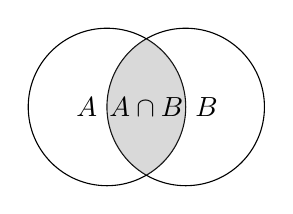
\begin{tikzpicture}
                    \draw (0,0) circle[radius=1cm];
                    \draw (1,0) circle[radius=1cm];
                    \begin{scope}
                        \clip (1,0) circle [radius=1]; % B の形でクリッピングする
                        \fill[gray, opacity=0.3] (0,0) circle [radius=1]; % スコープの中で A を塗りつぶす
                    \end{scope}
                    \node at (0,0) [anchor=east] {$A$};
                    \node at (1,0) [anchor=west] {$B$};
                    \node at (0.5,0) [anchor=center] {$A\cap B$};
                \end{tikzpicture}
                \caption{共通部分$A\cap B$のVenn図}
            \end{figure}
        \clearpage
        \subsection{直積集合}
            QuuノートIにおいて, 実数$\mathbb{R}$は数直線ととらえることができると説明した. 同様にして, 二つの数直線を直交させてできる
            平面についても, この平面上の各点と二つの数直線の値とを対応付けることができるだろう. これは, 関数のグラフを書く時にすでに
            (直接言及されていないだけで)学んだことである. この平面の各点は, 二つの集合$\mathbb{R},\mathbb{R}$の各要素を対にしたもの
            全てを集めた集合といえよう.
            \begin{figure*}[h]
                \centering
                \begin{tikzpicture}
                    \coordinate (P) at (1,2);
                    \draw[->] (-1,0) -- (3,0);
                    \draw[->] (0,-1) -- (0,3);
                    \node at (P) [anchor = west] {$(1,2)$};
                    \fill (P) circle[radius=0.1cm];
                    \draw[dashed] (1,0) -- (P);
                    \draw[dashed] (0,2) -- (P);
                    \node at (1,0) [anchor=north] {$1$};
                    \node at (0,2) [anchor=east] {$2$};
                    \node at (3,0) [anchor=west] {$x$};
                    \node at (0,3) [anchor=south] {$y$};
                \end{tikzpicture}
            \end{figure*}

            一般に, 二つの集合$A,B$に対して
            \begin{equation}
                A\times B =\{(a,b)\mid a\in A,b\in B\} \label{eq:集合論基礎:直積の定義}
            \end{equation}
            を$A$と$B$の\textbf{直積集合}\index{ちょくせきしゅうごう@直積集合}または単に\textbf{直積}\index{ちょくせき@直積}という. ここで, $(a,b)$は二つのもの$a,b$から作られる対となるもので, 
            これを\textbf{順序対}\index{じゅんじょつい@順序対}という. 順序対は集合と違って, $(a,b)\neq (b,a)$となる. つまり, 対の順序が違えばそれは違うものとみなす.
            二つの順序対$(a,b),(a',b')$が等しいのは$a=a',b=b'$となるときに限るとする. 

            直積を用いれば, 先ほど例で挙げた平面も$\mathbb{R}\times \mathbb{R}$と書けるとわかる. ただこの場合, 同一の集合の直積であるから
            簡単に$\mathbb{R}^2$と書くことにしよう. この記法は, 任意の集合$A$の直積$A\times A$についても用いられる. すなわち, $A\times A=A^2$である.

            直積の具体例を挙げよう. 例えば, $A=\{1,2,3\},B=\{2,3\}$とすると, $A\times B=\{(1,2),(1,3),(2,2),(2,3),(3,2),(3,3)\}$
            であり, $B\times A = \{(2,1),(2,2),(2,3),(3,1),(3,2),(3,3)\}$である. このように, 一般に直積では交換法則が成り立たない.

            直積$A\times B$において, $A,B$どちらか一方が空集合であれば順序対が存在しないので, この場合$A\times B$は空集合になる.\\

            今は二つの集合について, それぞれの要素から順序対を作っていた. これを$n$個の集合の場合に拡張しよう. $n$個の集合$A_1,A_2,\cdots,A_n$に対して, 
            それらの\textbf{直積集合}を
            \begin{equation}
                A_1\times A_2 \times \cdots \times A_n = \{(a_1,a_2,\cdot,a_n)\mid a_1\in A_1,a_2\in A_2,\cdots,a_n\in A_n\} \label{eq:集合論基礎:n個の直積の定義}
            \end{equation}
            によって定める. $(a_1,a_2,\cdots,a_n)$は順序対である. $n$個の場合でも二つの順序対が等しいのは, 並べられた各要素の値が等しい場合に限るとする.
            また, $A_1=A_2=\cdots=A_n=A$のとき, この直積集合を$A^n$とかく.\\

            直積は, もっと一般に集合系に対して定義される. しかし, 微分積分を学ぶ上では上記の定義で十分であるからここでは述べない.
            こちらも, 興味がある人は集合論の本を参考にしてほしい.
        \clearpage
        \subsection{写像}
            これまで扱ってきた関数は, 主に実数から実数に対応するものだった. 例えば, $f(x)=x^3$は, 全ての実数に対して定義され, 全ての実数に対応しているだろう.
            ここで議論したいのは, もっと一般に, 二つの集合間の対応である.
            
            二つの集合$X,Y$が与えられ, $X$の\underline{どの要素}に対しても, それぞれ$Y$の要素がただ一つ対応しているとき, この対応関係そのものを$X$から$Y$への\textbf{写像}\index{しゃぞう@写像}\footnote{対応関係自体を定義していないから, この定義は曖昧であるように感じる. この感覚は正常なものだ. 実際は, $X\times Y$の部分集合を対応関係と定義し, そのうち全ての$x\in X$に対して, $y\in Y$が一意的に存在するものを写像というのである.}と定義する.
            写像は, 関数や変換とも呼ばれたりするが, 全てまったくの同義語である. \footnote{関数は, 特に$X$が数の場合にいうようである.} $X$から$Y$の写像が$f$であることは, 次のように書かれる.
            \begin{equation}
                f:X\rightarrow Y \label{eq:集合論基礎:写像の書き方}
            \end{equation}
            このとき, $X$を$f$の\textbf{定義域}(始域)\index{しいき@始域}$Y$を\textbf{値域}(終域)\index{しゅういき@終域}という. また, 二つの写像$f:X\rightarrow Y, f':X'\rightarrow Y'$が\textbf{同じ写像である}\footnote{$A\subset X$に対して定義される$g:A\rightarrow Y$が任意の$x\in A$に対し, $f(x)=g(x)$であるとき, $g$を$f$の$A$の制限という. このとき$g=f\upharpoonright_A$とかく. また, $f$は$g$の拡張と呼ばれる.}とは, $X=X'\land Y=Y'$
            であって, $^\forall x\in X [f(x)=f'(x)]$であることをいう. このとき, $f=f'$とかく.

            $f:x\rightarrow y$によって, $x\in X$が$y\in Y$に対応することを$y=f(x)$とかく. このとき, $y$を$f$による$x$の\textbf{像}\index{ぞう@像}という. また, $x$を$f$による$y$の原像\index{げんぞう@原像}という.\\

            これまで扱ってきた関数の中には, $\sin(x^2)$のように, 関数の中に関数が入っているものがあった. これを合成関数といったわけだが, これを写像の場合にも考えてみる. すなわち, 集合$X,Y,Z$と, 
            二つの写像$f:X\rightarrow Y, g:Y\rightarrow Z$を考え, この合成写像なるものを考えてみよう. 写像$h:X\rightarrow Z$を, $h(x)=g(f(x))$として定める. この写像の各像は, $X$の要素を$Y$に飛ばし, 
            その像を$g$で$Z$の要素にとばしたものと一致する. これを\textbf{合成写像}\index{ごうせいしゃぞう@合成写像}といい, $g\circ f$とかく.
            
            合成写像に関しては, 交換法則は成り立たないが, 結合法則は成り立つ. すなわち
            \begin{equation}
                h\circ (g\circ f) = (h\circ g)\circ f \label{eq:集合論基礎:合成写像の結合法則}
            \end{equation}
            が成り立つ. ただし, $f,g,h$は, 集合$X,Y,Z,W$について, $f:X\rightarrow Y, g:Y\rightarrow Z, h:Z\rightarrow W$とする.
            \begin{proof}
                $x\in X$とする. このとき\[ [h\circ (g\circ f)](x)=h((g\circ f)(x))=h(g(f(x)))=(h\circ g)(f(x))=[(h\circ g)\circ f](x)\]
                が成り立つ. したがって等号が成り立つ.
            \end{proof}
            $f:X\rightarrow Y$を写像とする. $A\subset X$に対して, $\{f(a)\mid a\in A\}$を$f$による$A$の\textbf{像}\index{ぞう@像}といい, $f(A)$とかく. また, $B\subset Y$に対して, 
            $\{x\in X\mid f(x)\in B\}$を$f$による$B$の\textbf{逆像}\index{ぎゃくぞう@逆像}または\textbf{原像}\index{げんぞう@原像}といい, $f^{-1}(B)$と表す. 明らかに, $f(A)\subset Y,f^{-1}(B)\subset X$である.

            例えば, $f:\mathbb{R}\rightarrow \mathbb{R};x\mapsto x^2$\footnote{このように, 写像の像を具体的に$x\mapsto f(x)$と書くことがある.}として, $f([0,1])=[0,1]$である. 一方, $f^{-1}([0,1])=[-1,1]$である. 
            すなわち, この場合像と逆像は等しくない. 像も逆像も等しい例として, $f:\mathbb{R}\rightarrow \mathbb{R};x\mapsto x^3$がある. 先ほどと同じ部分集合の像を考えると$f([0,1])=[0,1]$であるし, $f^{-1}([0,1])=[0,1]$である.
            から, この場合確かに等しい.
            \clearpage
            像と逆像に関しては以下の公式が成り立つ. ただし, $f:X\rightarrow Y$とし, $A_1,A_2\subset X,B_1,B_2\subset Y$とする.
            \begin{align}
                f(A_1 \cup A_2)&=f(A_1)\cup f(A_2) \label{eq:集合論基礎:像の和}\\
                f(A_1 \cap A_2)&\subset f(A_1)\cap f(A_2) \label{eq:集合論基礎:像の積}\\
                f^{-1}(B_1 \cup B_2)&=f^{-1}(B_1)\cup f^{-1}(B_2) \label{eq:集合論基礎:逆像の和}\\    
                f^{-1}(B_1 \cap B_2)&=f^{-1}(B_1)\cap f^{-1}(B_2) \label{eq:集合論基礎:逆像の積}\\    
                A_1 &\subset f^{-1}(f(A_1)) \label{eq:集合論基礎:像の逆像}\\
                f(f^{-1}(B_1)) &\subset B_1 \label{eq:集合論基礎:逆像の像}\\
                f(A_1)-f(A_2) &\subset f(A_1-A_2) \label{eq:集合論基礎:像の差}\\
                f^{-1}(B_1)-f^{-1}(B_2) &= f^{-1}(B_1-B_2) \label{eq:集合論基礎:逆像の差}
            \end{align}
            これも像と逆像の定義から導出できるから, 各自で証明してほしい. ここでは, \eqref{eq:集合論基礎:像の和}と\eqref{eq:集合論基礎:像の逆像}のみ証明しよう.
            \begin{proof}[\eqref{eq:集合論基礎:像の和}の証明.]
                \begin{equation*}
                    f(A_1\cup A_2)=\{f(a)\mid a\in A_1\cup A_2\}=\{f(a)\mid a\in A_1\lor a\in A_2\}
                \end{equation*}
                であるから, $y\in f(A_1\cup A_2)$のとき, $y=f(a)$となる$a\in A_1$または$a\in A_2$が存在する. このときそれぞれ$y\in f(A_1),y\in f(A_2)$となるので
                $y\in f(A_1\cup A_2)\rightarrow y\in f(A_1)\cup f(A_2)$となる. 一方, $y\in f(A_1)\cup f(A_2)$のとき, $y\in f(A_1)$または$y\in f(A_2)$だから
                それぞれ$y=f(a)$となる$a\in A_1$もしくは$a\in A_2$が存在する. よって, $y\in f(A_1\cup A_2)$となるので, $y\in f(A_1)\cup f(A_2)\rightarrow y\in f(A_1\cup A_2)$である.
                従って, $f(A_1\cup A_2)=f(A_1)\cup f(A_2)$が示された.
            \end{proof}
            \begin{proof}[\eqref{eq:集合論基礎:像の逆像}の証明.]
                $a\in A_1$とする. このとき, 像の定義より$f(a)\in f(A_1)$が成り立つ. 一方逆像の定義から
                \begin{equation*}
                    f^{-1}(f(A_1))=\{x\in X\mid f(x)\in f(A_1)\}
                \end{equation*}
                であるから, (集合の$\mid$より右の条件を満たすことより)$a\in f^{-1}(f(A_1))$である. よって, $A_1\subset f^{-1}(f(A_1))$
            \end{proof}
            \eqref{eq:集合論基礎:像の逆像}の証明において重要なのは, $a\in X$としたときに$f(a)\in f(A_1)$であっても, $a\in A_1$とは\underline{限らない}という点である. 例を挙げると, $f(x)=x^2$のとき
            $f([0,1])=[0,1]$であったが, $x=-1\in [-1,0]$であっても, $f(x)=(-1)^2=1\in [0,1]$が成り立っている. すなわち, $f(x)\in f([0,1])$となる$x$は$[-1,0]$内にも存在している.\\

            一般の写像に関する性質は以上でほとんどであるが, これだと\eqref{eq:集合論基礎:像の逆像}のような包含関係しか得られない. できる限り$=$であってほしいのが心情だろう.
            そこで, 写像の中でもとくに``都合の良い''ものを考えよう.

            写像$f:X\rightarrow Y$について, 次のように定める.
            \begin{enumerate}
                \item $f(X)=Y$であるとき, $f$は\textbf{全射}\index{ぜんしゃ@全射}または\textbf{上への写像}\index{うえへのしゃぞう@上への写像}であるという.
                \item $x_1,x_2\in X$について, $x_1\neq x_2$ならば$f(x_1)\neq f(x_2)$であるとき, $f$は\textbf{単射}\index{たんしゃ@単射}または\textbf{1対1写像}\index{1たい1しゃぞう@1対1写像}であるという.
                \item $f$が全射かつ単射であるとき, $f$は\textbf{全単射}\index{ぜんたんしゃ@全単射}であるという.
            \end{enumerate}
            写像$f$が全単射であれば, \eqref{eq:集合論基礎:像の和}から\eqref{eq:集合論基礎:逆像の差}のうち$\subset$であるものは等号が成り立つようになる. 
            全単射である写像の例として, 一次関数$f(x)=ax+b\quad (a\neq 0)$がある. これが全単射であることは容易に確かめられるから, これも各自で確かめてみるとよいだろう.
            \clearpage
            任意の集合$X_1\subset X_2$に対し, $X_1$の各要素$x$に対して, $i(x)=x$となる写像$i:X_1\rightarrow X_2$を\textbf{包含写像}\index{ほうがんしゃぞう@包含写像}という. 特に, $X_1=X_2=X$であるとき, 
            \textbf{恒等写像}\index{こうとうしゃぞう@恒等写像}という. 恒等写像はよく$\mathrm{id}_X$と書かれる. 恒等写像は全単射である. これも明らかである.\\

            写像$f:X\rightarrow Y$が全単射のとき, どの$y\in Y$に対しても$y=f(x)$となる$x\in X$が一意に定まるはずである. そこで, $y\in Y$に対して, $y=f(x)$を満たす$x\in X$
            を対応させることで, $Y$から$X$への写像が定まる. この写像を$f^{-1}:Y\rightarrow X$とかき, $f$の\textbf{逆写像}\index{ぎゃくしゃぞう@逆写像}という. 先ほど定義した逆像と言葉が似ているが, 異なる概念であるから気を付けてほしい.

            逆写像に関する基本的な定理には, 以下のものがある.
            \begin{screen}
                $f:X\rightarrow Y,\quad g:Y\rightarrow X$を写像とする. このとき$g\circ f = \mathrm{id}_X$であれば, $f$は単射で$g$は全射である.
                特に, $f\circ g = \mathrm{id}_Y$であれば, $f,g$はともに全単射で$g$は$f$の逆写像である.
            \end{screen}
            \begin{proof}
                $g\circ f=\mathrm{id}_X$であるとする. このとき, $x_1,x_2\in X$について$f(x_1)=f(x_2)$であるとする. このとき写像の定義から$g(f(x_1))=g(f(x_2))$である. 
                ところで, $g(f(x))=(g\circ f)(x)=\mathrm{id}_X(x)=x$であるから, $x_1=x_2$である. すなわち, $f(x_1)=f(x_2)\rightarrow x_1=x_2$だから, 対偶を取れば
                $x_1\neq x_2\rightarrow f(x_1)\neq f(x_2)$となって, $f$の単射性が示された. 次に, $g$が全射であることを示す. $x\in X$とする. このとき, $y=f(x)$と置くと, 
                $g(y)=g(f(x))=x$である. すなわち, $X$の任意の要素に対して, 対応元$y\in Y$が存在するから, $g$は全射である. まったく同様にして, $f\circ g= \mathrm{id}_Y$
                であれば, $f$は全射で$g$は単射である. 従って, $f,g$は全単射である. $g$が$f^{-1}$なのは逆写像の定義から明らかであろう.
            \end{proof}
            実は, 上の定理において$g\circ f$が単射であれば$f$は単射であり, $g\circ f$が全射であれば, $g$も全射である.\footnote{このとき, $f:X\rightarrow Y,g:Y\rightarrow Z$であっても成り立つ.} これは上の証明をすこし変えるだけだから, 読者への演習問題としよう.\\

            集合の列$A_1,A_2,\cdots,A_n$を考えよう. これらは, 各添え字$1,2,\cdots,n$に対して, 集合$A_1,A_2,\cdots,A_n$が対応している状態であるから, 添え字の集合$\{1,2,\cdots,n\}$からある集合族への一つの写像$A$が
            与えられていると考えられる. このように, ある空でない添え字の集合$\Lambda$からある集合族への写像$A$のことを, $\Lambda$上の\textbf{集合系}\index{しゅうごうけい@集合系}といい, 
            \begin{equation}
                (A_\lambda\mid\lambda \in \Lambda),\quad (A_\lambda)_{\lambda\in\Lambda} \label{eq:集合論基礎:集合系の定義1}
            \end{equation}
            とかく. 実用上は, 集合系も集合族も拘泥せず同じ集合の集合と考えてもよい. そのため, \eqref{eq:集合論基礎:集合系の定義1}は以下のようにも書かれる.
            \begin{equation}
                \{A_\lambda\mid \lambda\in\Lambda\} \label{eq:集合論基礎:集合系の定義2}
            \end{equation}
            集合系に対して, 和集合と共通部分を以下のように定める.
            \begin{align}
                \bigcup_{\lambda\in \Lambda} A_\lambda = \{x\mid {}^\exists \lambda \in \Lambda,x\in A_\lambda\} \label{eq:集合論基礎:集合系の和集合}\\
                \bigcap_{\lambda\in \Lambda} A_\lambda = \{x\mid {}^\forall \lambda \in \Lambda,x\in A_\lambda\} \label{eq:集合論基礎:集合系の共通部分}
            \end{align}
            \eqref{eq:集合論基礎:集合系の和集合}および\eqref{eq:集合論基礎:集合系の共通部分}はそれぞれ$\bigcup \{A_\lambda\mid\lambda\in\Lambda\},\bigcap \{A_\lambda\mid\lambda\in\Lambda\}$と書かれることもある. また, $\Lambda=\{1,2,\cdots,n\}$のときは, $\displaystyle\bigcup_{k=1}^{n},\bigcap_{k=1}^{n}$
            の記号を用いることもある. とくに, $\Lambda = \mathbb{N}$であれば, 
            \begin{equation*}
                \bigcup_{n=1}^{\infty}A_n,\quad \bigcap_{n=1}^{\infty}A_n
            \end{equation*}
            とかいてもよい. 

            集合系の各集合$A_\lambda$が集合$X$の部分集合であるとき, この集合系を$X$の\textbf{部分集合系}\index{ぶぶんしゅうごうけい@部分集合族}という. $\{A_\lambda\mid \lambda\in\Lambda\}$を$X$の部分集合系とする.
            このとき, 次の\textbf{De Morganの法則}\index{De Morganのほうそく@De Morganの法則}が成り立つ.
            \begin{align}
                \left(\bigcup_{\lambda\in\Lambda}A_\lambda\right)^c=\bigcap_{\lambda\in\Lambda}(A_\lambda)^c \label{eq:集合論基礎:一般のドモルガン1}\\
                \left(\bigcap_{\lambda\in\Lambda}A_\lambda\right)^c=\bigcup_{\lambda\in\Lambda}(A_\lambda)^c \label{eq:集合論基礎:一般のドモルガン2}
            \end{align}
            \eqref{eq:集合論基礎:一般のドモルガン2}は\eqref{eq:集合論基礎:一般のドモルガン1}からすぐでるから, \eqref{eq:集合論基礎:一般のドモルガン1}のみ示す.
            \begin{proof}
                \begin{equation*}
                    x\in \left(\bigcup_{\lambda\in\Lambda}A_\lambda\right)^c \leftrightarrow \lnot [{}^\exists\lambda\in\Lambda,x\in A_\lambda]\leftrightarrow{}^\forall\lambda\in\Lambda,x\not\in A_\lambda\leftrightarrow{}^\forall\lambda\in\Lambda,x\in (A_\lambda)^c\leftrightarrow \bigcap_{\lambda\in\Lambda}(A_\lambda)^c
                \end{equation*}
                より等号が成り立つ.
            \end{proof}
            最後に, 集合系の極限にあたるものを定義しよう. $\mathbb{N}$を添え字の集合系とする集合系$\{A_n\mid n\in\mathbb{N}\}$に対して, 
            \begin{equation}
                \limsup_{n\to\infty}A_n=\bigcap_{k=1}^{\infty}\bigcup_{n=k}^\infty A_n \label{eq:集合論基礎:集合のlimsup}
            \end{equation}
            を\textbf{上極限集合}\index{うえきょくげんしゅうごう@上極限集合}という. 上極限集合は, 無限個の$A_n$に属す要素全てを集めた集合である. また, 
            \begin{equation}
                \liminf_{n\to\infty}A_n=\bigcup_{k=1}^{\infty}\bigcap_{n=k}^\infty A_n \label{eq:集合論基礎:集合のliminf}
            \end{equation}
            を\textbf{下極限集合}\index{したきょくげんしゅうごう@下極限集合}という. 下極限集合は, 有限個の$A_k$だけ除いて, それ以外を全て集めた集合である. 

            まず基本的なのは, 次の包含関係である.
            \begin{equation}
                \liminf_{n\to\infty}A_n\subset\limsup_{n\to\infty}A_n \label{eq:集合論基礎:limsupとliminfの包含関係}
            \end{equation}
            本によってはこの関係を明らかと書くようである. しかし, 私個人がこれを単に`明らか'とするのは納得がいかないから, 証明を与える.
            \begin{proof}
                すぐにわかることとして, $\displaystyle \bigcap_{n=k-1}^\infty A_n\subset\bigcap_{n=k}^\infty A_n$がある. したがって, 各$i\in\mathbb{N}$について, 
                \begin{equation*}
                    \liminf_{n\to\infty} A_n=\bigcup_{k=1}^{\infty}\bigcap_{n=k}^\infty A_n=\bigcup_{k=i}^{\infty}\bigcap_{n=k}^\infty A_n
                \end{equation*}
                が成り立つ. 実際, $i$が大きくなることで生じる和集合の`漏れ'は, すべて$k\geq i$以降の$\bigcap_{k} A_n$に含まれている.
                また, $\displaystyle \bigcap_{n=k}^\infty A_n\subset A_k$であることもすぐわかる. したがって, 
                \begin{equation*}
                    \bigcup_{k=i}^{\infty}\bigcap_{n=k}^\infty A_n\subset \bigcup_{k=i}^{\infty}A_k\Rightarrow \bigcap_{i=1}^\infty\bigcup_{k=i}^{\infty}\bigcap_{n=k}^\infty A_n\subset \bigcap_{i=1}^\infty\bigcup_{k=i}^{\infty}A_k=\limsup_{n\to\infty}A_n
                \end{equation*}
                であり, 左辺は$\displaystyle \bigcap_{i=1}^\infty\bigcup_{k=i}^{\infty}\bigcap_{n=k}^\infty A_n=\bigcup_{k=1}^{\infty}\bigcap_{n=k}^\infty A_n=\liminf_{n\to\infty}A_n$だから, $\displaystyle\liminf_{n\to\infty}A_n\subset\limsup_{n\to\infty}A_n$.
            \end{proof}
            \eqref{eq:集合論基礎:limsupとliminfの包含関係}において, 特に等式が成り立つ場合, これを\textbf{極限集合}\index{きょくげんしゅうごう@極限集合}といって, 
            \begin{equation}
                \lim_{n\to\infty}A_n=\limsup_{n\to\infty}A_n=\liminf_{n\to\infty}A_n \label{eq:集合論基礎:極限集合の定義}
            \end{equation}
            とかく. これらの概念はLebesgue積分論において重要である.
            \clearpage


        \clearpage
        \subsection{濃度}
                集合の個数と写像の関係について考えてみたい. 例えば, $\{1,2,3\}$と$\{p,i,e\}$という集合は, 個数が等しい. このとき, 二つの集合間に全単射が存在している. 例えば, $1\mapsto p,2\mapsto i,3\mapsto e$
                とすれば, これは明らかに全単射である. このように有限集合で個数が等しいときは全単射が存在している. 逆に, 二つの有限集合間に全単射が存在すれば, それらの要素数は等しいともいえるだろう.
                問題は無限集合である. 無限集合と有限集合の要素数が違うのはすぐわかるが, 無限集合同士ではどうだろうか. そもそも要素数が無限である場合, 要素数の比較などできるのだろうか.
                このような疑問を解消するために, 集合の濃度というものを考えてみよう. 二つの集合$A,B$の\textbf{濃度が等しい}\index{のうどがひとしい@濃度が等しい}とは, $A$から$B$への
                全単射が存在することである. このとき, $A\sim B$とかく. これは有限集合で考えていた集合の要素数の比較を拡張したものと考えてもよいだろう. 実際先ほどみたように, 有限集合で
                要素数が等しいときは, 全単射が存在するから, 濃度も等しいし, その逆も成り立っている. この濃度を用いて, 自然数の集合$\mathbb{N}$と偶数全体の集合$E$を比較してみよう.
                これは簡単で, 写像$f:\mathbb{N}\rightarrow E,n\mapsto 2n$を考えると, この写像は全単射であるから, $\mathbb{N}\sim E$が成り立つ. しかし, この結果は直感に反しているように感じているだろう.
                厳密性を欠いた表現をすれば, この結果は「自然数と偶数の`個数'が等しい」ということを意味しているのだから. 面白い例はほかにもある. 例えば, $\mathbb{N}\sim\mathbb{Z}$が成立する.
                これも直感に反しているようだが, 全単射は構成できてしまう. この全単射については, 演習問題で考えてもらうことにしよう.

                集合$A,B,C$について, 以下が成り立つ.
                \begin{enumerate}\renewcommand{\labelenumi}{(\arabic{enumi})}
                    \item $A\sim A$
                    \item $A\sim B$ならば$B\sim A$
                    \item $A\sim B$かつ$B\sim C$ならば$A\sim C$
                \end{enumerate}
                \begin{proof}以下それぞれ証明を述べる. どれも示すことは, 全単射の存在である.
                    \begin{enumerate}\renewcommand{\labelenumi}{(\arabic{enumi})}
                        \item 恒等写像$\mathrm{id}_A$を考えればよい.
                        \item 仮定より$A\rightarrow B$の全単射が存在して, 全単射の逆写像を考えればこれは$B\rightarrow A$の全単射である.
                        \item $A\rightarrow B$の全単射と$B\rightarrow C$の全単射の合成写像を考えれば, これは全単射である.
                    \end{enumerate}
                \end{proof}
                二つの全単射の合成写像が全単射であることは直感的に明らかであるが, 厳密に証明をしておこう. より強い主張である以下の補題を示そう.
                \begin{screen}
                    写像$f:X\rightarrow Y,g:Y\rightarrow Z$について, 以下が成立する.
                    \begin{enumerate}\renewcommand{\labelenumi}{(\roman{enumi})}
                        \item $f,g$ともに単射であれば$g\circ f$も単射.
                        \item $f,g$ともに全射であれば$g\circ f$も全射.
                    \end{enumerate}
                \end{screen}
                \begin{proof}以下に証明を述べる.
                    \begin{enumerate}\renewcommand{\labelenumi}{(\roman{enumi})}
                        \item $x_1,x_2\in X,x_1\neq x_2$とする. $y_1=f(x_1),y_2=f(x_2)$と置くと, $f$の単射性から$y_1\neq y_2$である. また, $g$の単射性から$g(y_1)\neq g(y_2)$である. 
                        従って, $(g\circ f)(x_1)=g(f(x_1))=g(y_1)\neq g(y_2)=g(f(x_2))=(g\circ f)(x_2)$だから, $g\circ f$は単射.
                        \item 示すことは, $(g\circ f)(X)=Z$である. $f,g$は全射であるから$f(X)=Y,g(Y)=Z$が成立する. すなわち, 任意の$z\in Z$に対し, $z=g(y)$となる$y\in Y$および$y=f(x)$となる$x\in X$が存在する.
                        よって, $z=g(y)=g(f(x))=(g\circ f)(x)\in (g\circ f)(X)$が成り立つ. これより$Z\subset (g\circ f)(X)$であり, 写像の定義より$Z\supset (g\circ f)(X)$だから$Z=(g\circ f)(X)$, よって$g\circ f$は全射.
                    \end{enumerate}
                \end{proof}
                全射の証明は, 以前述べた全射を示す証明とすこしやり方が違うように見えるだろう. 実際にはどちらのスタイルで証明してもらっても構わない. 個人的には, 今回の証明のほうがわかりやすい気がする.
                なおこの補題より, 全単射同士の合成写像が全単射であることは明らかであろう.\\

                全ての集合の濃度は互いに等しいとは限らない. この事実は重要である. 例えば以下が成り立つ.
                \begin{screen}
                    \[\mathbb{N}\nsim \mathbb{R}\]
                \end{screen}
                これはCantorによって示された. 彼の有名な\textbf{対角線論法}\index{たいかくせんろんぽう@対角線論法}と呼ばれるアイデアを見てみよう.
                \begin{proof}
                    背理法\footnote{証明すべき命題を否定した命題をもとに論理を導き, 矛盾を見つけることで元の命題を示す方法.}で示す. $\mathbb{N}\sim\mathbb{R}$であれば, 全単射$f:\mathbb{N}\rightarrow \mathbb{R}$が存在する.
                    このとき(すべての)実数$f(n)$について, 10進法による無限小数展開を行うと, $f(n)=a_{n0}.a_{n1}a_{n2}\cdots a_{nn}\cdots$となる. ただし, 各$a_{nm}\quad(m=1,2,...)$が0から9までの整数,$a_{0n}\in \mathbb{Z}$で, 整数や有限小数は小数部分に0を続けるとする.
                    例を挙げる. 例えば,$3.1415...$なら$a_{n0}=3,a_{n1}=1,a_{n2}=4,...$となる. $2.4$なら$a_{n0}=2,a_{n1}=4,a_{n2}=a_{n3}=\cdots=0$である. $n=1$から書き並べると以下のようになる.
                    \begin{align*}
                        f(1)&=a_{10}.\bm{a_{11}}a_{12}a_{13}\cdots\\
                        f(2)&=a_{20}.a_{21}\bm{a_{22}}a_{23}\cdots\\
                        f(3)&=a_{30}.a_{31}a_{32}\bm{a_{33}}\cdots\\
                        \vdots
                    \end{align*}
                    小数部分の太字を見てほしい. この対角の数字を用いて, 新たな無限小数を作る. 具体的には, 各$a_{nn}$について
                    \begin{equation*}
                        b_n=\left\{\begin{array}{lc}
                            1 & (a_{nn}は偶数)\\
                            2 & (a_{nn}は奇数)
                        \end{array}\right.
                    \end{equation*}
                    である$b_n$を用いて, 無限小数$b=0.b_{11}b_{22}b_{33}\cdots$をつくる. 重要なのは, 必ず$b_{n}\neq a_{nn}$となることである. この$b$は明らかに$b\in{\mathbb{R}}$であるが, 
                    すべての$n\in \mathbb{N}$に対して, $f(n)\neq b$である. なぜなら, どの$n$についても小数第$n$位の数字が$b$と異なるからである.
                    これは, $f$が全単射(全射)であることに矛盾する.
                \end{proof}
                自然数全体の集合$\mathbb{N}$と濃度が等しい集合を\textbf{可算集合}\index{かさんしゅうごう@可算集合}という. また, 有限集合と可算集合を合わせて\textbf{高々可算集合}\index{たかだがかさんしゅうごう@高々可算集合}
                という.\\

                集合の濃度を表す記号等を導入しておこう. 集合$A$に対して, $A$の\textbf{濃度}\index{のうど@濃度}を$|A|$または$\mathrm{card}A$を書く.
                集合の濃度とは, 濃度が等しい集合を集めた組のことである. 要素数$n$の有限集合の濃度は$n$とかく. また, 可算集合の濃度は$\aleph_0$(アレフ・ゼロ)とかき,  
                $\mathbb{R}$の濃度は$2^{\aleph_0}$とかく. 例えば, $|\varnothing|=0,|\mathbb{Z}|=\aleph_0$である.
                \clearpage

                我々が次に望むのは, 濃度を大小で比較できるようになることだろう. 集合$A,B$について, $A$から$B$への単射が存在するが, $B$から$A$への
                単射が存在しないとき, $A$は$B$より\textbf{濃度が小さい}\index{のうどがちいさい@濃度が小さい}, または, $B$は$A$より\textbf{濃度が大きい}\index{のうどがおおきい@濃度が大きい}という.
                $B$から$A$への単射が存在したときは何も言えないのか, と疑問に思うかもしれない. 実は, \textbf{Bernsteinの定理}\index{Bernsteinのていり@Bernsteinの定理}によって, $A$から$B$への単射と$B$から$A$への単射が存在するとき, 濃度が等しいことが濃度が等しいことが保障される.
                証明はここでは述べないから, 興味がある人は調べてみるとよい.\\

                最も重要なのは, 有理数の集合$\mathbb{Q}$が可算集合であることである. そのためにはまず, 二つの補題を示さなければならない.
                \begin{screen}
                    集合$A,B$が$A\subset B$であれば, $A$から$B$への単射が存在する.
                \end{screen}
                \begin{proof}
                    包含写像$i:A\rightarrow B$を考えると, これは明らかに単射であるから, 示された.
                \end{proof}

                \begin{screen}
                    $\mathbb{Z}^2$は可算集合である.
                \end{screen}
                \begin{proof}
                    $\mathbb{Z}=\{(m,n)\mid m,n\in\mathbb{Z}\}$は, 平面$\mathbb{R}^2$上の格子点の集合であるから, 下図のように対応をつけることで, $\mathbb{Z}^2=\{a_1,a_2,\cdots,a_n\cdots\}$
                    とできる. したがって, $\mathbb{Z}^2$は可算集合である.
                    \begin{figure}[h]
                        \centering
                        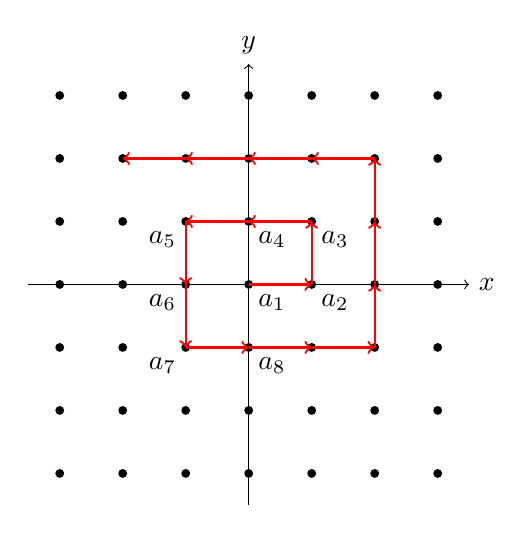
\begin{tikzpicture}[scale=0.8]
                            % 格子点を描画
                            \foreach \x in {-3,...,3} {
                                \foreach \y in {-3,...,3} {
                                    \fill (\x,\y) circle (2pt);
                                }
                            }

                            % 軸を描画
                            \draw[->] (-3.5,0) -- (3.5,0) node[right] {$x$};
                            \draw[->] (0,-3.5) -- (0,3.5) node[above] {$y$};

                            % 編番号の経路を矢印で描画
                            \draw[thick,->,red] (0,0) -- (1,0);
                            \draw[thick,->,red] (1,0) -- (1,1);
                            \draw[thick,->,red] (1,1) -- (0,1);
                            \draw[thick,->,red] (0,1) -- (-1,1);
                            \draw[thick,->,red] (-1,1) -- (-1,0);
                            \draw[thick,->,red] (-1,0) -- (-1,-1);
                            \draw[thick,->,red] (-1,-1) -- (0,-1);
                            \draw[thick,->,red] (0,-1) -- (1,-1);
                            \draw[thick,->,red] (1,-1) -- (2,-1);
                            \draw[thick,->,red] (2,-1) -- (2,0);
                            \draw[thick,->,red] (2,0) -- (2,1);
                            \draw[thick,->,red] (2,1) -- (2,2);
                            \draw[thick,->,red] (2,2) -- (1,2);
                            \draw[thick,->,red] (1,2) -- (0,2);
                            \draw[thick,->,red] (0,2) -- (-1,2);
                            \draw[thick,->,red] (-1,2) -- (-2,2);

                            % 編番号を数列形式で表示
                            \node[below right] at (0,0) {$a_1$};
                            \node[below right] at (1,0) {$a_2$};
                            \node[below right] at (1,1) {$a_3$};
                            \node[below right] at (0,1) {$a_4$};
                            \node[below left] at (-1,1) {$a_5$};
                            \node[below left] at (-1,0) {$a_6$};
                            \node[below left] at (-1,-1) {$a_7$};
                            \node[below right] at (0,-1) {$a_8$};
                        \end{tikzpicture}
                        \caption{$a_1=(0,0)$として, 反時計回りに対応付けていく.}
                    \end{figure}
                \end{proof}

                準備が整ったので, $\mathbb{Q}$が可算集合であることを示そう.
                \begin{proof}
                    まず, $\mathbb{N}\subset \mathbb{Q}$より, $\mathbb{N}$から$\mathbb{Q}$への単射が存在する. 次に, $r\in \mathbb{Q}$は, 既約分数として$r=p/q\hspace{1mm}(p\in\mathbb{Z},b\in\mathbb{N})$
                    の形にかける(整数$n$については, $q=1$として, $x=x/1$とかく). このとき, 
                    \begin{equation*}
                        f:\mathbb{Q}\rightarrow\mathbb{Z}^2,\frac{p}{q}\mapsto (p,q)
                    \end{equation*}
                    は単射であるから, $\mathbb{Z}^2$が可算であるので$\mathbb{Z}^2$から$\mathbb{N}$への全単射が存在する. 以上より, $\mathbb{Q}$から$\mathbb{N}$への単射が存在するから, Bernsteinの定理より
                    $\mathbb{Q}\sim \mathbb{N}$である.
                \end{proof}
                \clearpage
                最後に, 可算集合の部分集合は高々可算集合であることを示そう.
                \begin{proof}
                    可算集合を$A$とする. $B\subset A$は有限集合か無限集合である. 有限集合であれば, それは高々可算集合であるから, $B$は無限集合であるとする.
                    仮定より, 全単射$f:A\rightarrow \mathbb{N}$が存在する. よって, $f(B)=N\subset \mathbb{N}$と置くと, $B\sim N$である.
                    $B$が無限集合であるから, $N$も無限集合である. したがって, 自然数の無限部分集合$N$が可算であることを示せばよい.
                    写像$g:N\rightarrow\mathbb{N}$を考える. $g(n)$は集合$\{m\in N\mid m\leq n\}$の要素数とする. このとき, $g$は全単射である.
                    \begin{enumerate}
                        \item 単射の証明.\\
                        $n_1,n_2\in N,n_1\neq n_2$とする. 対称性から$n_1<n_2$と仮定してもよい. このとき, $m\leq n_1$をみたす$m\in N$は$m\leq n_2$も満たし, 
                        後者の場合は$m=n_2$も条件を満たすから, $g(n_1)<g(n_2)$. したがって, $g(n_1)\neq g(n_2)$だから$g$は単射.
                        \item 全射の証明.\\
                        $n\in \mathbb{N}$とする. $N$は無限部分集合であるから, $n=g(k)$となる$k\in N$は存在する. ($N$の要素にはいくらでも大きい値がある.)
                        すなわち, $n\in g(N)$であるから, $\mathbb{N}\subset f(N)$. よって, $g$は全射.
                    \end{enumerate}
                    これより, $N$から$\mathbb{N}$への全単射が存在するから, $N\sim\mathbb{N}$. ゆえに, $B\sim \mathbb{N}$
                \end{proof}

        \clearpage
        \subsection{実数の連続性}
    \clearpage
    \section{行列と行列式}
        ベクトルのイメージとその和・差について. 内積についても述べる. 外積はベクトル解析のときに述べる. 続いて, 行列についてその定義を述べ, 和・差・積について述べる.
        転置行列と逆行列についても述べる. 行列式は, 一般の定義を述べ, その後2x2と3x3について計算方法を述べる. 余因子展開についてその計算方法を述べる.
    \clearpage
    \section{偏微分}
        多変数関数をまず具体例で挙げ, その後偏微分について解説する.二変数テイラー展開及び積分記号下の微分まで述べる.
    \clearpage
    \section{多重積分}
        多重積分についてまず二重積分についてその定義を話す. かんたんな計算ののちに三重積分も述べる. その後, 変数返還について, 一次変換の場合について厳密な証明を行い, 
        それ以外は感覚的なものにとどめる.
    \clearpage
    
    \part{ベクトル解析}
    \vspace{\stretch{1}}
    \begin{screen}
        ベクトル解析は, 理工系の学生にとって馴染み深いものと聞く. たいていの物理科と電気科の学生は, 電磁気学にて顔を合わせることになるだろう.
        よく電磁気学は, ベクトル解析をふんだんに用いるから難しいと言われているが, 少なくともベクトル解析単体で見ればそこまで難しいものではない. 
        そして何よりベクトル解析は楽しいものである. ここでは, まずベクトルについての基礎知識について述べた後, ベクトル値関数についてその微分積分を定義する.
        その後, 空間上の曲線および曲面の解析についてすこし述べ, ベクトル解析の顔ともいえる微分演算子について述べる.
        電磁気学ではよく用いられるGaussの発散定理およびStokesの定理についても扱う. 
    \end{screen}
    \clearpage
    \section{ベクトルの性質と演算}
        数学基礎で述べたことと多少重複するが, 内積, 外積およびそれらの性質を述べる. スカラー三重積とベクトル三重積も述べる.
    \clearpage
    \section{ベクトル値関数とその微分}
        ベクトル値関数について述べたのち, それらの微分積分を定義する. ただし, 積分は定義のみで深く触れない.
    \clearpage
    \section{曲線の解析}
        曲線について解析する. 平面曲線について述べて, 空間曲線でも議論する. Frenet-Serretの公式まで.
    \clearpage
    \section{曲面論入門}
        曲面について解析する. 基本量を導出し, Gauss曲率と平均曲率を紹介する.
    \clearpage
    \section{微分演算子}
        ベクトル場とスカラー場について説明する. その後各微分演算子について述べる.
    \clearpage
    \section{線積分と面積分}
        線積分と面積分について定義を述べる. Gaussの定理とStokesの定理について述べ, 電磁気学への応用をしてみる.
    \clearpage

    \part{複素解析}
    \vspace{\stretch{1}}
    \begin{screen}
        複素解析は, 数学の中で最も美しい理論の一つと言われる. 複素関数(複素数から複素数へ対応させる関数)に対して, 正則という概念が定義できる.
        正則性とはかんたんに言えば微分可能性のことなのであるが, 驚くべきことにこの正則性を満たせば,それらを微分した関数も正則性を保つのである. 
        これらの性質を含め, 正則関数の解析の基本となるのはCauchyの積分定理である. ここでは, 複素数についてその基本的な性質を述べ, 複素関数および
        複素微分について定義し, 複素平面上での積分を述べる. その後, Cauchyの積分定理をはじめとする, 正則関数に関する多くの定理を証明する.
        その中には実積分の計算に対してたいへん有効な留数定理もある. この理論の美しさをじっくり味わってほしい.
    \end{screen}
    \clearpage
    \section{複素数}
        複素数についてその基礎知識を述べる. 複素平面上の領域も. De Moivreの定理まで述べる.
    \clearpage
    \section{複素関数とその微分}
        複素関数について定義し, その性質について簡単に述べる. Cauchy-Riemannの方程式も述べる. 初等関数についても述べる.
    \clearpage
    \section{複素線積分}
        かんたんな線積分の計算をして, Cauchyの積分定理を述べる. Cauchyの積分公式やGoursatの定理などの多数定理を述べる. 最大値の原理
        については証明させる?
    \clearpage
    \section{級数}
        複素数列について, その収束等を定義し, 複素級数についても定義する. ベキ級数やTaylor展開, Maclaurin展開についても述べる.
        Laurent展開を重点的に扱う.特異点とその分類も述べる.Picardの大定理は入れない. 無限遠点のLaurent展開も述べる.
    \clearpage
    \section{留数定理}
        留数について定義を述べて, 留数定理を示す. その後, 実積分の計算を行う. 無限遠での留数についても述べる.
    \clearpage
    \section{解析接続}
        解析接続について簡単な例を挙げ, 一致の定理を証明して, 解析接続の一意性について説明する.
    \clearpage
    \section{Riemann面}
        余裕があれば,多価関数とRiemann面についてすこしだけ述べる.
    \clearpage

    \part{相対性理論}
    \vspace{\stretch{1}}
    \begin{screen}
        相対性理論...それはかの天才物理学者Einsteinが作り上げた物理学の中で最も美しい理論である. 理科や宇宙が好きな
        小学生であればほとんどの人があこがれていたものであると思うし, それ以外の人でも, 相対性理論から導かれる不思議な
        世界(双子のパラドクスなど)について聞いたことがある人も多いと思う. 相対性理論が美しいといわれるその所以は, たった一つ
        の物理的要請に真摯に従って計算することで, 重力場の基礎方程式(いわゆる, Einstein方程式)までたどり着けるところであろう. 
        その要請とは, 「物理学の法則は, 座標系に依存しない形式に書かれなければならない」という, 実に自然な, 当然ともいえる要請である.
        この要請から, さまざまな相対性理論の世界が開けることには, ただただ驚嘆するばかりである.\\
        相対性理論は, 一般に非常に難しいといわれている. 確かに, 相対性理論, 特に一般相対性理論を真に理解するには, 数学のRiemann幾何学について熟知していないといけないだろう.
        しかし, 特殊相対性理論に限って言えば, かんたんな力学の知識さえあれば(一部を除いて)理解することができる. また, 一般相対性理論に関しても, 重力場の方程式を導くだけであれば
        必要なRiemann幾何学の知識も特別難しいものではないのである.\\
        ここでは, 特殊相対性理論について, よく子供向けの科学本などに載っている事象を中心に数学的に理解していく.
        また, 一般相対性理論についても軽く触れる.
    \end{screen}
    \clearpage
    \section{特殊相対論入門}
        Galilei変換についてと慣性系について述べる. 光速度不変の原理について, 実験結果から述べ, Lorentz変換を導出する. 
         Minkowski時空上の距離, 世界間隔について説明する. このときLorentz変換に対して不変であることを述べる.
        固有時間などについても述べる.
    \clearpage
    \section{パラドクスの解決}
        パラドクスをここで解決する. 双子のパラドクスと時計のパラドクス
    \clearpage
    \section{数学的準備}
        ベクトルやテンソルについて, かんたんに定義する.
    \clearpage
    \section{相対論的力学}
        相対論上で力学を展開する. $E=mc^2$の導出や変分原理についても扱う. 双子のパラドクスを変分原理を用いて解決する.
    \clearpage
    \section{一般相対論への展望}
        Riemann幾何学の$ds^2$を紹介して, 等価原理について$\Gamma=0$であることを紹介する.
    \clearpage

    \part{Lebesgue積分入門}
    \vspace{\stretch{1}}
    \begin{screen}
        積分好きなら一度は聞いたことがあるのが, このLebesgue積分である. Lebesgue積分は, 単なる数学の枠を飛び越えて, 
        物理学や工学で必須のFourier解析や, 偏微分方程式, また確率論などのいたるところに顔を出す非常に重要な概念である.
        それにもかかわらず, このLebesgue積分はなかなかに難しく, 習得にも時間がかかる. これはLebesgue積分が素朴なRiemann積分と違って
        内容がいささか抽象的であることが原因であるように思える. さらに, 集合論に関する知識も必要であり, 学ぶための敷居が高い.
        そこでここでは, Lebesgue積分論のうち, 特に重要であるものを選択して系統的に学べるよう, 構成を工夫した. 
        端的に言えば, 極限と積分の順序交換ができる単調収束定理へ最短経路で学べるようになっているのである.
        なおこのLebesgue積分は, Riemann積分と対照的に, しばしばグラフを横に切る積分であると説明される. 実際まちがってはないが, 
        実際にLebesgue積分を学んでいると, 横に切っているというイメージはあまりないので注意してほしい.
    \end{screen}
    \clearpage
    \section{可測空間}
        集合体, $\sigma$-集合体の定義を述べ, 可測空間を定義する. 部分集合族から生成される$\sigma$-集合体や可測分割等も述べる.
    \clearpage
    \section{測度}
        集合関数の定義および測度の定義を述べる. 様々な測度の例を述べる. 測度の基本的な性質についても示す. $\mu$-零集合
        についても触れ, 完備測度空間を定義する. 完備測度への測度の拡張が存在し, しかもそれが一意であることを述べる.
    \clearpage
    \section{可測関数}
        可測関数の定義, 基本的性質を述べる. 単関数を定義し, 任意の正なる可測関数に対して, 収束する単関数の単調増加列が存在することを示す.
        ほとんど到る所(almost everywhere)についても触れる.
    \clearpage
    \section{積分}
        積分を定義し, 諸性質を述べる. 関数が連続であれば, Riemann積分とLebesgue測度に対する積分(Lebesgue積分)が一致することも述べる.
    \clearpage
    \section{収束定理}
        Lebesgueの有界収束定理を証明する. 適用例などをみてその威力を体感する.
    \clearpage
    \part{終わりに}
        \clearpage
    \printindex
\end{document}